% Preamble
\documentclass[11pt]{article}

% Packages
\usepackage{amsmath}
\usepackage[italian]{babel}
\usepackage{graphics}
\usepackage{graphicx}
\usepackage{csvsimple}
\usepackage{hyperref}
\graphicspath{{../results/}}


% Document
\title{Problemi di Render : Parallel Programming for Machine Learning}
\author{Lorenzo Baiardi, Thomas Del Moro}
\date{10 12 2023}

\begin{document}

    \maketitle
    \clearpage

    %\tableofcontents
    %\clearpage

    \section{Introduzione}\label{sec:introduzione}
    In questo elaborato verificheremo l'efficacia dell'utilizzo di metodi di parallelizzazione in problemi comuni,
    studiandone i risultati, la velocità e i tempi di esecuzione.

    \section{Analisi del problema}\label{sec:analisi-del-problema}
    Il problema che abbiamo deciso di valutare è quello del compositing tra piani tramite l'utilizzo della libreria
    grafica OpenCV\@.
    Ogni piano avrà 4 canali di colore (RGBA), e per ogni piano verranno disegnati n cerchi.
    Durante la fase di sommatoria dei piani, viene applicato un effetto trasparenza in base alla posizione del piano
    all'interno della sommatoria.
    Una volta che vengono sommati tutti i piani, tramite operazione di compositing, verrà restituita una matrice
    risultante con l'immagine finale.
    I parametri utilizzati all'interno del progetto variano in base ai test effettuati.

    \begin{figure}[h!]
        \begin{minipage}{0.32\textwidth}
            \centering
            
\includegraphics[width=\textwidth]{img/seq/10000}
            \caption{Sequenziale}
        \end{minipage}%
        \hfill
        \begin{minipage}{0.32\textwidth}
            \centering
            
\includegraphics[width=\textwidth]{img/par/10000}
            \caption{OMP}
        \end{minipage}%
        \hfill
        \begin{minipage}{0.32\textwidth}
            \centering
            
\includegraphics[width=\textwidth]{img/cuda/10000}
            \caption{CUDA}
        \end{minipage}
        \caption{Immagini di esempio con 10000 piani}\label{fig:example-images}
    \end{figure}

    \section{Parallelizzazione}\label{sec:parallelizazzione}
    Per poter parallelizzare il problema abbiamo deciso di utilizzare due approcci differenti, nel primo caso abbiamo
    utilizzato la libreria OPENMP al variare del numero di thread e nel secondo caso abbiamo utilizzato il linguaggio di
    programmazione CUDA per il calcolo parallelo su scheda grafica\@.
    Entrambi i metodi verranno analizzati e confrontati tra loro per verificare quale sia il più efficiente.
    Il metodo preso in considerazione per la parallelizzazione è:
    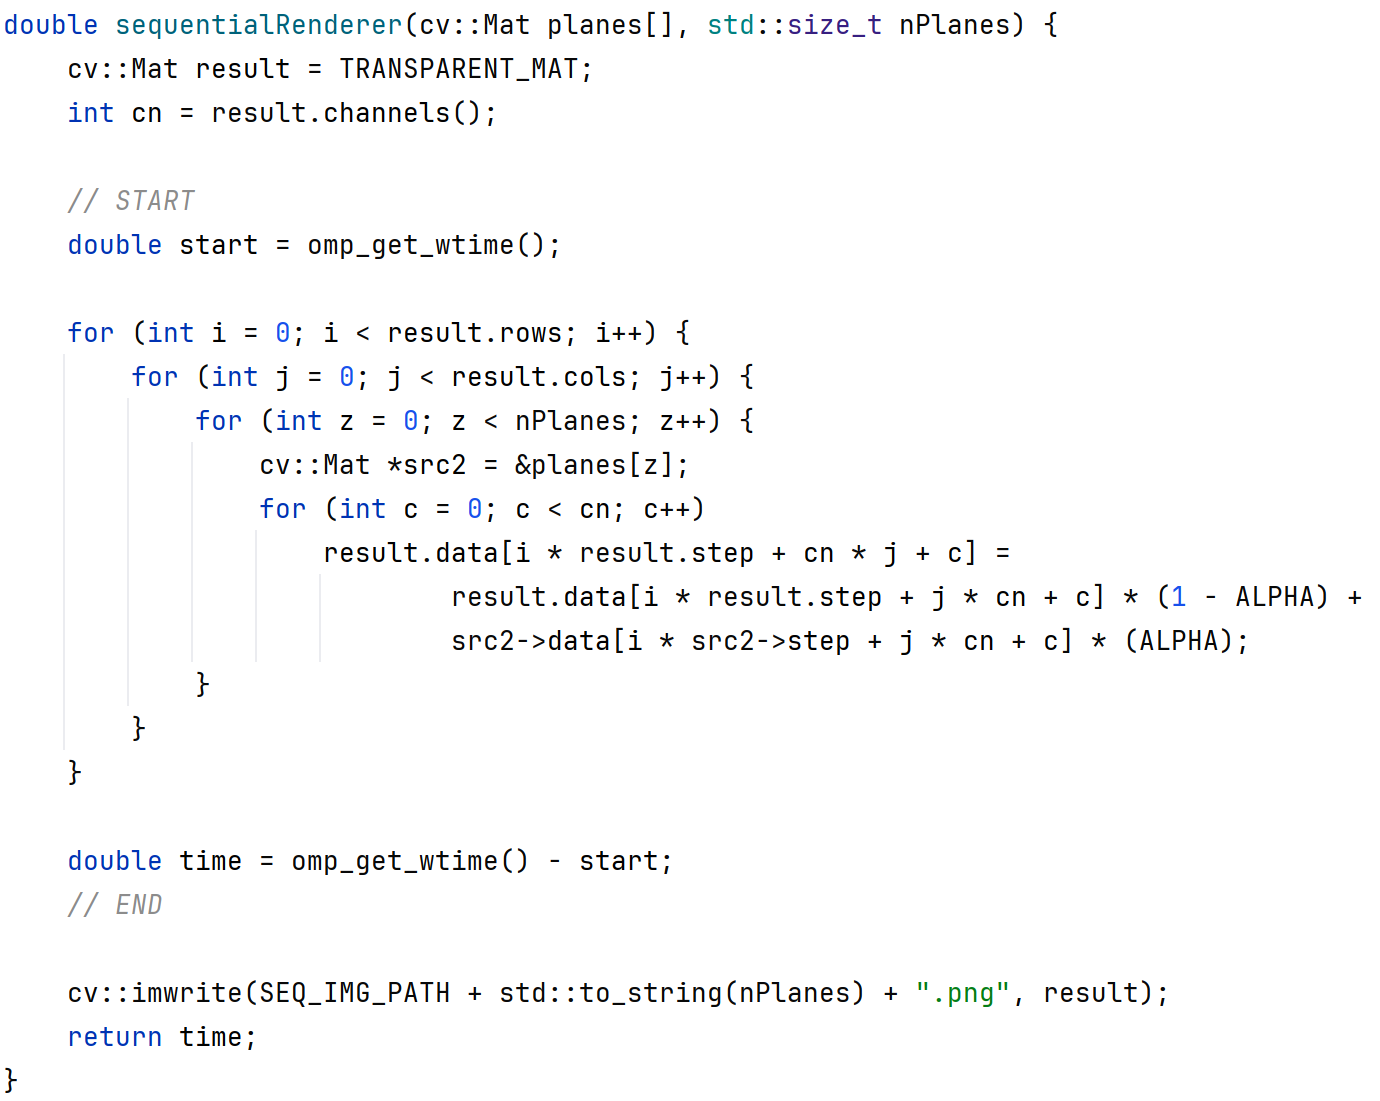
\includegraphics[width=\textwidth]{../documentation/img/code (1)}

    \subsection{OPENMP}\label{subsec:openmp}
    L'idea di fondo è quella che ogni thread gestisca la sommatoria di un singolo pixel per ogni matrice, in
    modo da preservare l'ordinamento dei piani ma aumentandone la velocità di render.
    Di conseguenza ogni thread calcolerà il pixel risultante e successivamente, al termine di esso, passerà
    al successivo pixel.
    All'interno dell'esperimento varieremo il numero di thread che il calcolatore potrà utilizzare per la
    parallelizzazione per verificarne l'efficienza.
    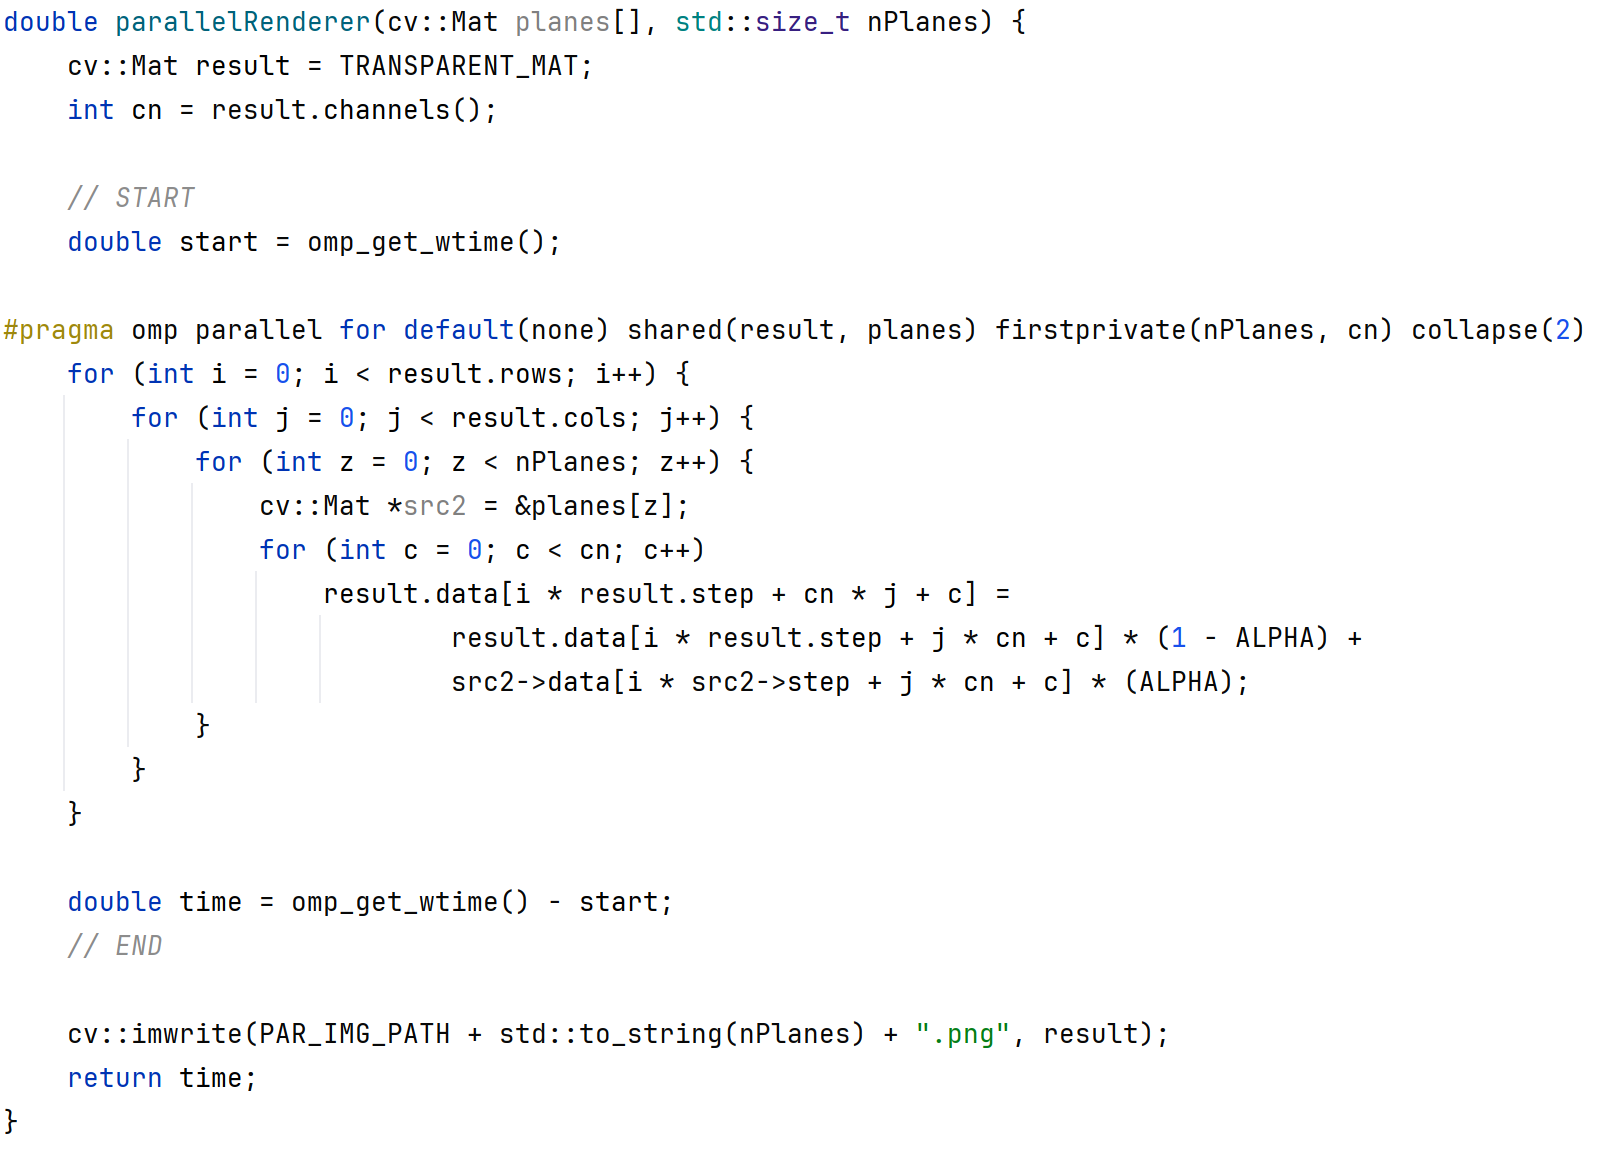
\includegraphics[width=\textwidth]{../documentation/img/code (2)}

    \subsection{CUDA}\label{subsec:cuda}
    In questo caso la parte di parallelizzazione si svilupperà principalmente nel calcolo di grid e block da utilizzare.
    Anche in questo caso, ogni thread gestirà un singolo pixel per ogni matrice, in modo da preservare
    l'ordinamento dei piani ma sfruttando la potenza di calcolo della scheda grafica.
    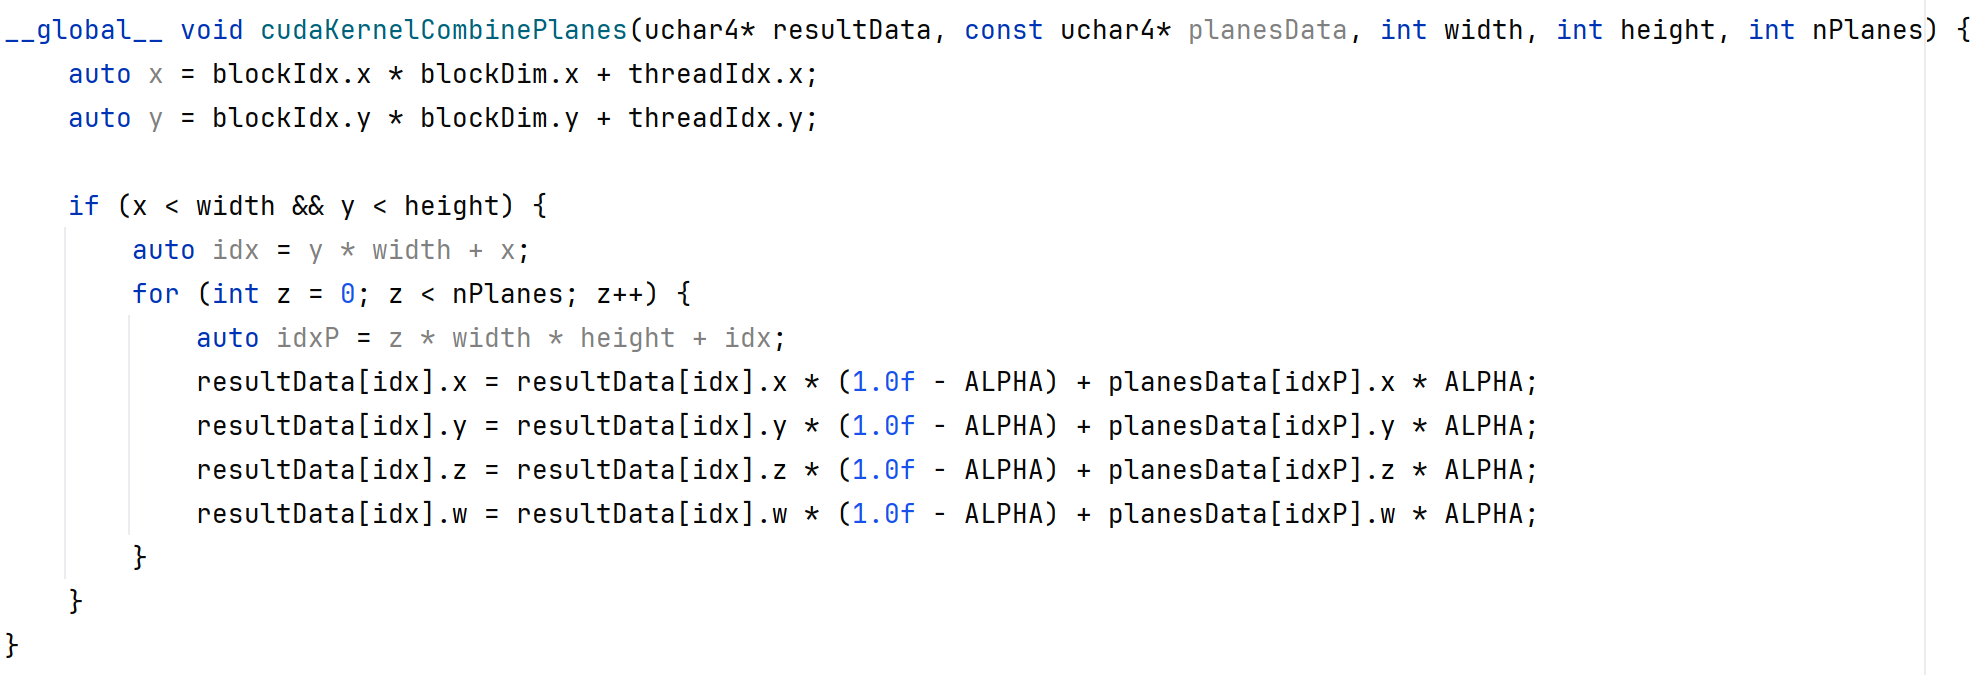
\includegraphics[width=\textwidth]{../documentation/img/code (3)}
    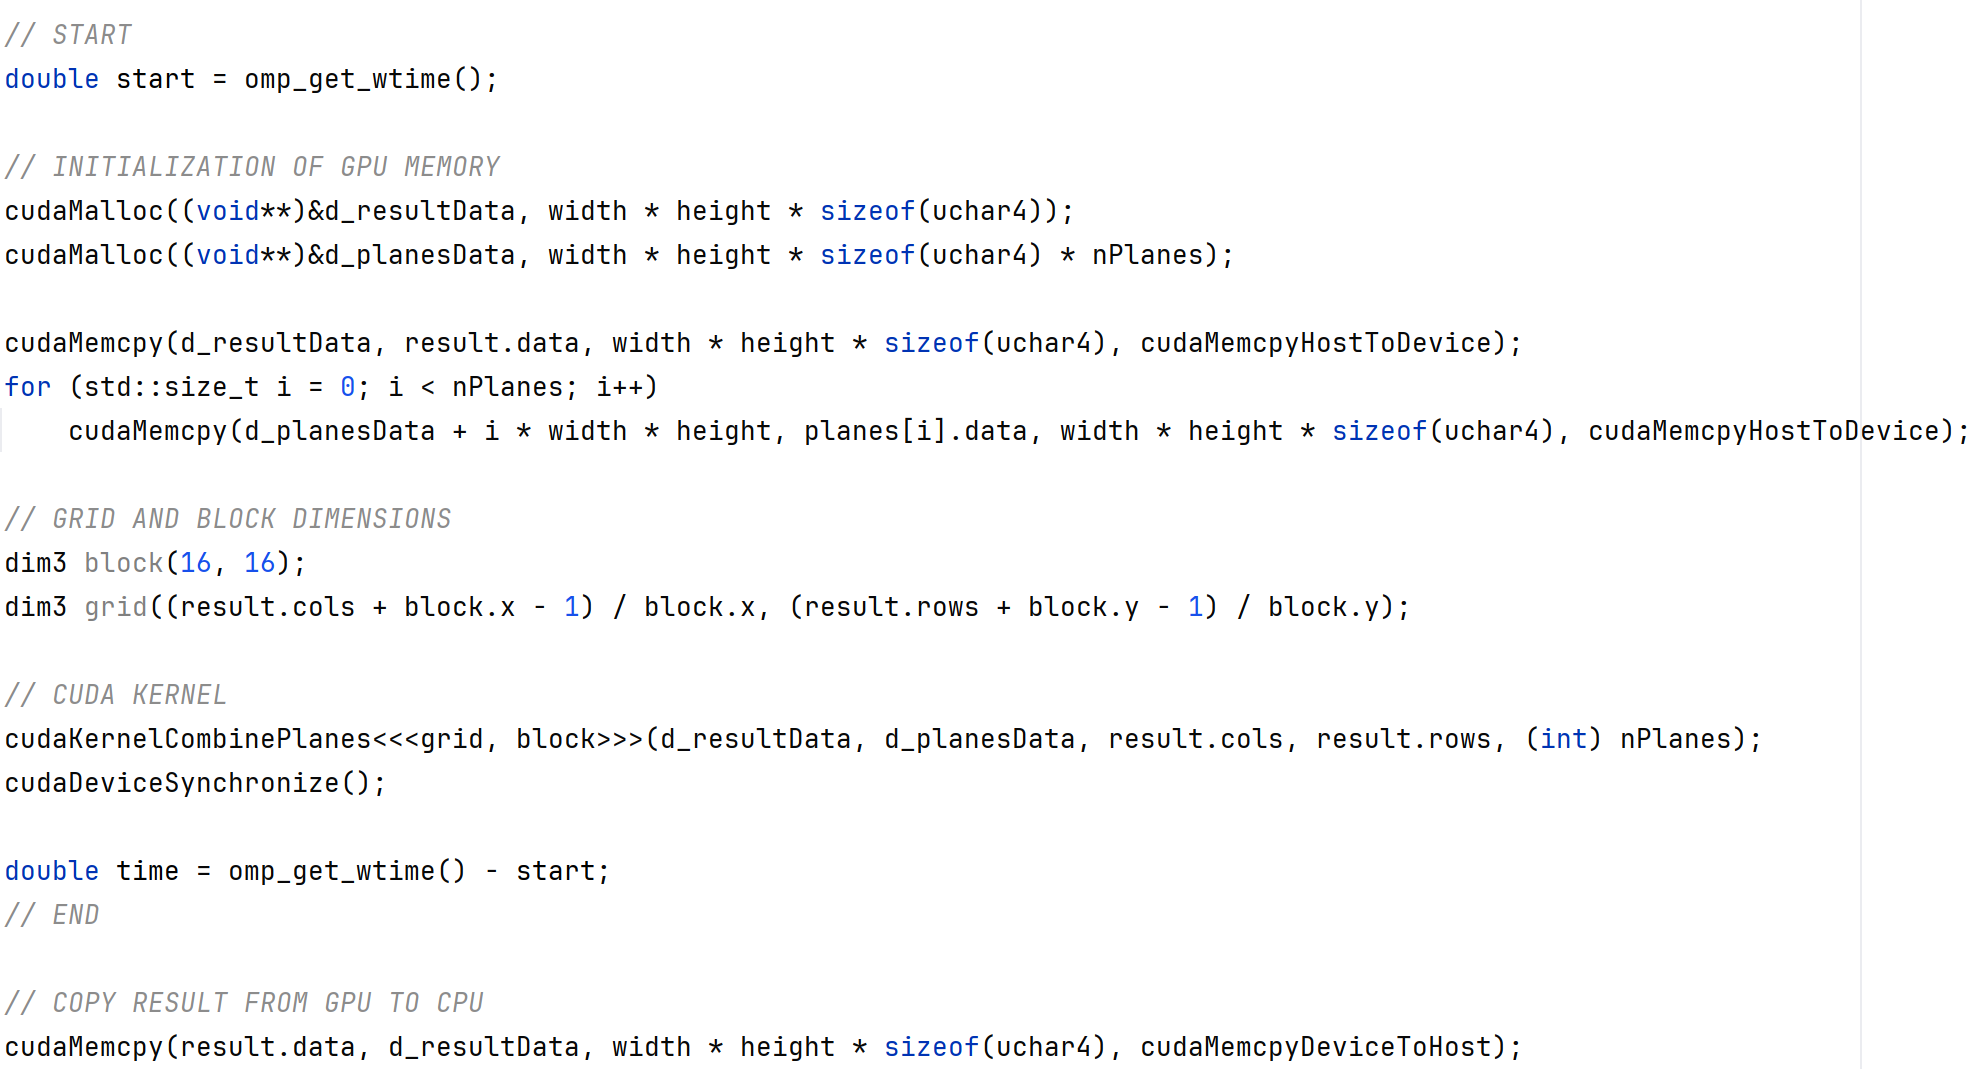
\includegraphics[width=\textwidth]{../documentation/img/code (4)}

    \section{Tests}\label{sec:tests}
    I test sono stati effettuati N volte variando il numero e le dimensioni dei piani, il numero di cerchi disegnati
    per piano e limitando il numero di thread da poter eseguire alla volta.
    I cerchi che dovranno essere disegnati sono generati precedentemente all'esecuzione del test, verificando
    così se i risultati delle varie operazioni riportino una soluzione identica.

    \subsection{Risultati}\label{subsec:plots}
    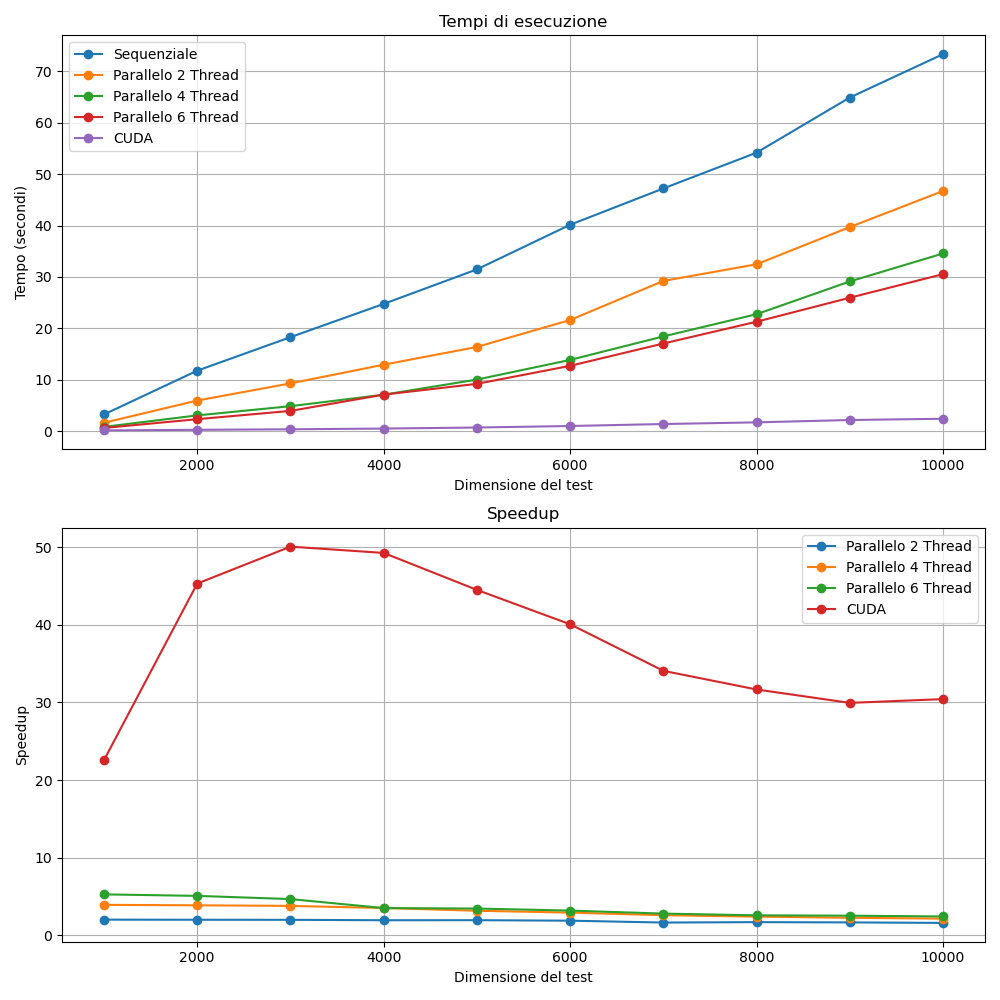
\includegraphics[width=\textwidth]{plots/results}
    %\csvautotabular{../results/csv/test.csv}

    \begin{table}
        \begin{minipage}{0.49\textwidth}
            \begin{tabular}{|c|c|c|c|}
            \hline
            test & seq & par & speedUp \\
            \hline
            1000 & 3.251 & 1.632 & 1.992 \\
            2000 & 11.766 & 5.952 & 1.977 \\
            3000 & 18.281 & 9.291 & 1.968 \\
            4000 & 24.751 & 12.929 & 1.914 \\
            5000 & 31.467 & 16.377 & 1.921 \\
            6000 & 40.148 & 21.621 & 1.857 \\
            7000 & 47.208 & 29.218 & 1.616 \\
            8000 & 54.180 & 32.463 & 1.669 \\
            9000 & 64.901 & 39.696 & 1.635 \\
            10000 & 73.335 & 46.719 & 1.570 \\
            \hline
            \end{tabular}
            \caption{2 thread}
        \end{minipage}
        \hfill
        \begin{minipage}{0.49\textwidth}
            \begin{tabular}{|c|c|c|c|}
                \hline
                test & seq & par & speedUp \\
                \hline
                1000 & 3.251 & 0.834 & 3.900 \\
                2000 & 11.766 & 3.063 & 3.841 \\
                3000 & 18.281 & 4.856 & 3.764 \\
                4000 & 24.751 & 7.092 & 3.490 \\
                5000 & 31.467 & 10.029 & 3.138 \\
                6000 & 40.148 & 13.859 & 2.897 \\
                7000 & 47.208 & 18.426 & 2.562 \\
                8000 & 54.180 & 22.748 & 2.382 \\
                9000 & 64.901 & 29.120 & 2.229 \\
                10000 & 73.335 & 34.563 & 2.122 \\
                \hline
            \end{tabular}
            \caption{4 thread}
        \end{minipage}\label{tab:table1}
    \end{table}

    \begin{table}
        \begin{minipage}{0.49\textwidth}
            \begin{tabular}{|c|c|c|c|}
            \hline
            test & seq & par & speedUp\\
            \hline
            1000 & 3.251 & 0.619 & 5.251 \\
            2000 & 11.766 & 2.327 & 5.055 \\
            3000 & 18.281 & 3.937 & 4.643 \\
            4000 & 24.751 & 7.101 & 3.486 \\
            5000 & 31.467 & 9.200 & 3.420 \\
            6000 & 40.148 & 12.705 & 3.160 \\
            7000 & 47.208 & 17.049 & 2.769 \\
            8000 & 54.180 & 21.285 & 2.545 \\
            9000 & 64.901 & 25.955 & 2.501 \\
            10000 & 73.335 & 30.540 & 2.401 \\
            \hline
            \end{tabular}
            \caption{6 thread}
        \end{minipage}
        \hfill
        \begin{minipage}{0.49\textwidth}
            \begin{tabular}{|c|c|c|c|}
                \hline
                test & seq & cuda & speedUp\\
                \hline
                1000 & 3.251 & 0.144 & 22.558 \\
                2000 & 11.766 & 0.260 & 45.332 \\
                3000 & 18.281 & 0.365 & 50.098 \\
                4000 & 24.751 & 0.502 & 49.288 \\
                5000 & 31.467 & 0.707 & 44.521 \\
                6000 & 40.148 & 1.002 & 40.084 \\
                7000 & 47.208 & 1.385 & 34.083 \\
                8000 & 54.180 & 1.710 & 31.675 \\
                9000 & 64.901 & 2.167 & 29.948 \\
                10000 & 73.335 & 2.410 & 30.433 \\
                \hline
            \end{tabular}
            \caption{CUDA}
        \end{minipage}\label{tab:table2}
    \end{table}

    \section{Conclusioni}\label{sec:conclusioni}
    In conclusione, possiamo vedere come l'operazione di parallelizzazione CUDA risulti il più efficiente, a
    discapito però nel avere a disposizione una scheda grafica NVDIA\@.
    Nonostante ciò, anche la parallelizzazione tramite OPENMP risulta molto efficiente rispetto alla formulazione
    sequenziale.

\end{document}